\documentclass[fleqn]{article}

\usepackage{arxiv}

% \usepackage[style=authoryear-comp, % Citation marks as [Jef65]
%             natbib=true,      % Natbib-style cite macros \citeauthor &c.
%             hyperref=true,    % Cites in pdf are links to bib
%                               % (hyperref conf.)
%             maxnames=3,       % truncate name lists if more than 2
%                               % names appear
%             doi=false,        % no doi's
%             url=false,        % no url's
%             sortcites=false,  % do NOT sort cites in the style of the
%                               % bibliography
%             %backref=true     % insert backrefs in reference section
%             ]{biblatex}
\usepackage{mypackages}
\bibliography{~/Desktop/icloud/MyRefGlobal}
\usepackage{mycommands}

\usepackage[utf8]{inputenc} % allow utf-8 input
\usepackage[T1]{fontenc}    % use 8-bit T1 fonts
\usepackage{hyperref}       % hyperlinks
\usepackage{url}            % simple URL typesetting
\usepackage{booktabs}       % professional-quality tables
\usepackage{amsfonts}       % blackboard math symbols
\usepackage{nicefrac}       % compact symbols for 1/2, etc.
\usepackage{microtype}      % microtypography
\usepackage{cleveref}       % smart cross-referencing
\usepackage{lipsum}         % Can be removed after putting your text content
\usepackage{graphicx}
\usepackage{doi}

\usepackage{float}

% Statistical models based on LLM predictions
% LLMs fuel statistical models for full distributional predictions of human experimental data
% Large language models for full distributional predictions of human experimental data
% Statistical modeling with predictors from large language models
\title{Beyond the best guess: Distributional predictions from large language models for human forced-choice data}

% Here you can change the date presented in the paper title
%\date{September 9, 1985}
% Or remove it
\date{}

\newif\ifuniqueAffiliation
% Uncomment to use multiple affiliations variant of author block
% \uniqueAffiliationtrue

\ifuniqueAffiliation % Standard variant of author block
  \author{ Michael Franke\thanks{Use footnote for providing further
		information about author (webpage, alternative
		address)---\emph{not} for acknowledging funding agencies.} \\
	Department of Linguistics\\
	University of Tübingen\\
	\texttt{michael.franke@uni-tuebingen.de} \\
	%% examples of more authors
	\And
	Polina Tsvilodub\thanks{Use footnote for providing further
		information about author (webpage, alternative
		address)---\emph{not} for acknowledging funding agencies.} \\
	Department of Linguistics\\
	University of Tübingen\\
	\texttt{polina.tsvilodub@gmail.com} \\
	\And
	Fausto Carcassi\thanks{Use footnote for providing further
		information about author (webpage, alternative
		address)---\emph{not} for acknowledging funding agencies.} \\
	Department of Linguistics\\
	University of Tübingen\\
	\texttt{fausto.carcassi@gmail.com} \\
	%% \AND
	%% Coauthor \\
	%% Affiliation \\
	%% Address \\
	%% \texttt{email} \\
	%% \And
	%% Coauthor \\
	%% Affiliation \\
	%% Address \\
	%% \texttt{email} \\
	%% \And
	%% Coauthor \\
	%% Affiliation \\
	%% Address \\
	%% \texttt{email} \\
}
\else
% Multiple affiliations variant of author block
\usepackage{authblk}
\renewcommand\Authfont{\bfseries}
\setlength{\affilsep}{0em}
% box is needed for correct spacing with authblk
% \newbox{\orcid}\sbox{\orcid}{\includegraphics[scale=0.06]{orcid.pdf}}
\author{Michael Franke, Polina Tsvilodub, Fausto Carcassi}
\affil{Department of Linguistics\\University of Tübingen\\
\texttt{[michael.franke|polina.tsvilodub|fausto.carcassi]@uni-tuebingen.de}}
\fi

% running right header
\renewcommand{\headeright}{}
% small title under big title
\renewcommand{\undertitle}{}
\renewcommand{\shorttitle}{Statistical modeling with LLM predictors}

%%% Add PDF metadata to help others organize their library
%%% Once the PDF is generated, you can check the metadata with
%%% $ pdfinfo template.pdf
\hypersetup{
pdftitle={Statistical modeling with LLM predictors},
pdfsubject={},
pdfauthor={Michael Franke, Polina Tsvilodub, Fausto Carcassi},
pdfkeywords={statistical models, language use, large language models, Bayesian data analysis, reference games},
}

\begin{document}
\maketitle

\begin{abstract}
	{\textcolor{gray}{fill me}}
\end{abstract}


% keywords can be removed
% \keywords{First keyword \and Second keyword \and More}

%%%%%%%%%%%%%%%%%%%%%%%%%%%%%%%%%%%%%%%%%%%%%%%%%%
\section{Introduction}
\label{sec:introduction}
%%%%%%%%%%%%%%%%%%%%%%%%%%%%%%%%%%%%%%%%%%%%%%%%%%

The invention of deep neural transformer architectures \citep{VaswaniShazeer2017:Attention-is-Al} enabled a new generation of powerful large language models (LLMs) \citep{DevlinChang2019:BERT:-Pre-train,ChungHou2022:Scaling-Instruc,OpenAI2023:GPT-4-Technical,TouvronLavril2023:LLaMA:-Open-and} which excel on standard benchmarks and promise to serve as foundation models for a vast and diverse set of applications \citep{BommasaniHudson2021:On-the-opportun}, especially when augmented with supervised fine-tuning  \citep{ChungHou2022:Scaling-Instruc} and reinforcement learning from human \citep{StiennonOuyang2022:Learning-to-sum} or other \citep{BaiKadavath2022:Constitutional-} feedback.
Recently an increasing number of diverse applications has gone beyond using LLMs out-of-the-box, i.e., based on their single-run input-output behavior, and instead utilize LLMs as a part of a larger computational process.
Examples aimed at improving output quality include sophisticated prompting \citep{LiuLiu2022:Generated-Knowl}, structured reasoning or ``neuro-symnolic AI'' \citep{CreswellShanahan2022:Selection-Infer}, or applications of LLMs as scoring functions in open-ended applications \citep{ZhangLehman2023:OMNI:-Open-ende}.
Other work, uses LLMs as part of bigger programs to build towards something more akin to explanatory cognitive models \citep{WongGrand2023:From-Word-Model}.
\mf{enlarge briefly, include more references}

For all of these applications, it is crucial to understand what LLMs can or cannot reliable do.
The prevalent approach towards understanding the performance of LLMs relies on benchmark testing which usually consists in assessing the accuracy of LLM predictions in tasks where a designated ``true answer'' exists, averaged over many instances of this task.
Benchmark-driven assessments are very useful to systematically study the effects of scale, e.g., in an engineering-oriented context \citep[e.g.,][]{srivastava2023-BIGbench}.
Other recent work is more psychologically oriented and asks to what extent LLM performace is ``human-like.''
LLM performance is therefore compared to human choice behavior in psychological experiments to investigate whether LLMs predict patterns of human answer behavior qualitatively \citep[e.g.,][]{BinzSchulz2023:Using-cognitive,Hagendorff2023:Machine-Psychol,ShiffrinMitchell2023:Probing-the-psy}.
Notably, some work goes even further and asks whether LLMs can also make adequate \emph{quantitative predictions}.
For example, work at the interface between NLP and computational psycholinguistics \citep{MarvinLinzen2018:Targeted-Syntac,HuGauthier2020:A-Systematic-As} has evolved into investigations of whether quantitative predictions by LLMs match quantitative aspects in human experimental data, such as measures of (self-paced) reading times \citep{WilcoxVani2021:A-Targeted-Asse} or the amplitude of common EEG signals like the N400 component \citep{LindborgRabovsky2021:Meaning-in-brai}.

This work seeks to extend the investigation in the human-likeness of LLM predictions even further, by exploring whether LLM-derived measures can feed into probabilistic models predicting the full distribution of human answers in a forced-choice tasks.

\begin{itemize}
  \item distributional predictions are more informative, so beneficial for ``understanding'' and for ``applications''
  \item for ``understanding LLMs'' more informative, richer predictions can be more diagnostic about LLM capabilities (risks and potentials)
  \item reliable full-distributional predictions from LLMs can be useful in applications, e.g., relative scoring based on elusive intuitive concepts like ``relevance'' or ``interestingness''
\end{itemize}

%%%%%%%%%%%%%%%%%%%%%%%%%%%%%%%%%%%%%%%%%%%%%%%%%%
\section{Motivation: Why care for distributional predictions?}
\label{motivation}
%%%%%%%%%%%%%%%%%%%%%%%%%%%%%%%%%%%%%%%%%%%%%%%%%%

The prevalent approach to assessing LLM performance based on benchmark-testing quantifies accuracy for a task based on a ``winner-takes-all'' (WTS) strategy.
Let $\set{I_{1}, \dots, I_{m}}$ be $m$ be instances all belonging to the same task, or items belonging to the same (logical) condition in a behavioral experiment.
% For human observers, these items are interchangeable, all exemplifying the same conceptual problem.
Each item $I_{k} = \tuple{x_{k}, \tuple{y_{k1}, \dots, y_{kl}}}$ consists of an input prompt $x_{k}$, which is a string of text, and $l$ choice alternatives $\tuple{y_{k1}, \dots, y_{kl}}$, all of which are strings as well, possibly composed of $|y_{ki}|$ words, $y_{ki} = w_{ki1}, \dots, w_{ki|y_{ki}|}$.
The most obvious \emph{item-level score} an (autoregressive) LLM provides for each choice option $y_{ki}$ is its log-probability:
%
\begin{align*}
  S\left( y_{ki}, x_{k} \right) = \log P_{\text{LLM}} \left(y_{ki} \mid x_{k} \right) =  \sum_{j=1}^{|y_{ki}|} \log P_{\text{LLM}} \left(w_{kij} \mid x_{k}, w_{ki1}, \dots, w_{ki(j-1)} \right)  \,.
\end{align*}
%
The WTS approach considers item $I_{k}$ to be answered correctly if the designated ``goal answer'' $y_{ki}$ is among the options that maximize the item-level score.
The accuracy of the LLM on the given task is the proportion of items in which the correct answer is selected.

While generally a pragmatic and useful approach, there are several reasons why going beyond the best guess can be beneficial.
Consider first a high-level conceptual argument.
If task performance is categorical (in the most extreme case: binary), somewhere along the path from a numerical item-level score to accuracy a discontinuity has to be introduced.
Every such discontinuity bottleneck entails loss of information.
As this information might be useful, discontinuity should ideally happen as late as possible; or even better: not at all, unless it is irrelevant.
Consequently, the question becomes: when is the additional information inherent in the scores (not) relevant for assessing LLM performance?

Imagine that there are two options, and that the goal answer is a small $\epsilon$ better in 80\% of the $m$ items, and otherwise worse.
The WTS strategy predicts an accuracy of 0.8.
This number is useful as a performance measure for applications in which the LLM is used in exactly the way the WTS strategy describes, e.g., any implementation which is outcome equivalent to greedy decoding with rejection sampling on a domain that contains only the available options.
For such a case, it never matters how much worse the goal answer is scored in the 20\% of the cases where it is not the maximum.
As only the best option will be chosen, that information is irrelevant.
But if an application uses anything other than greedy-like responses, the accuracy score of 0.8 may be misleading.
If the remaining 20\% of the items are such that the non-goal option is almost infinitely better, it would be chosen under a pure sampling strategy with virtual certainty, so the accuracy for choosing the goal answer in such an application scenario would around 0.4.\footnote{The probability of the second option in the 80\% of items where the goal answer is slightly better is 0.5 in the limit of $\epsilon \rightarrow 0$, and it is virtually 1 in the remaining 20\%.}
This is a categorical shift from predominantly goal answer to predominantly non-goal answer.
The argument holds equally if numbers for the two options are reversed, so that there is no way of saying which of the two accuracy scores would in principle be more favorable for selecting the goal answers.
Two things matter:
(i)
whether the LLM would be more likely used in cases where greedy-like evaluation is required; and
(ii)
what the nature of the item-level variation is.

\bigskip

\mf{to be continued}




%%%%%%%%%%%%%%%%%%%%%%%%%%%%%%%%%%%%%%%%%%%%%%%%%%
\section{Experiment: Reference games}
\label{experiment-reference-games}
%%%%%%%%%%%%%%%%%%%%%%%%%%%%%%%%%%%%%%%%%%%%%%%%%%

\begin{figure}
  \centering

  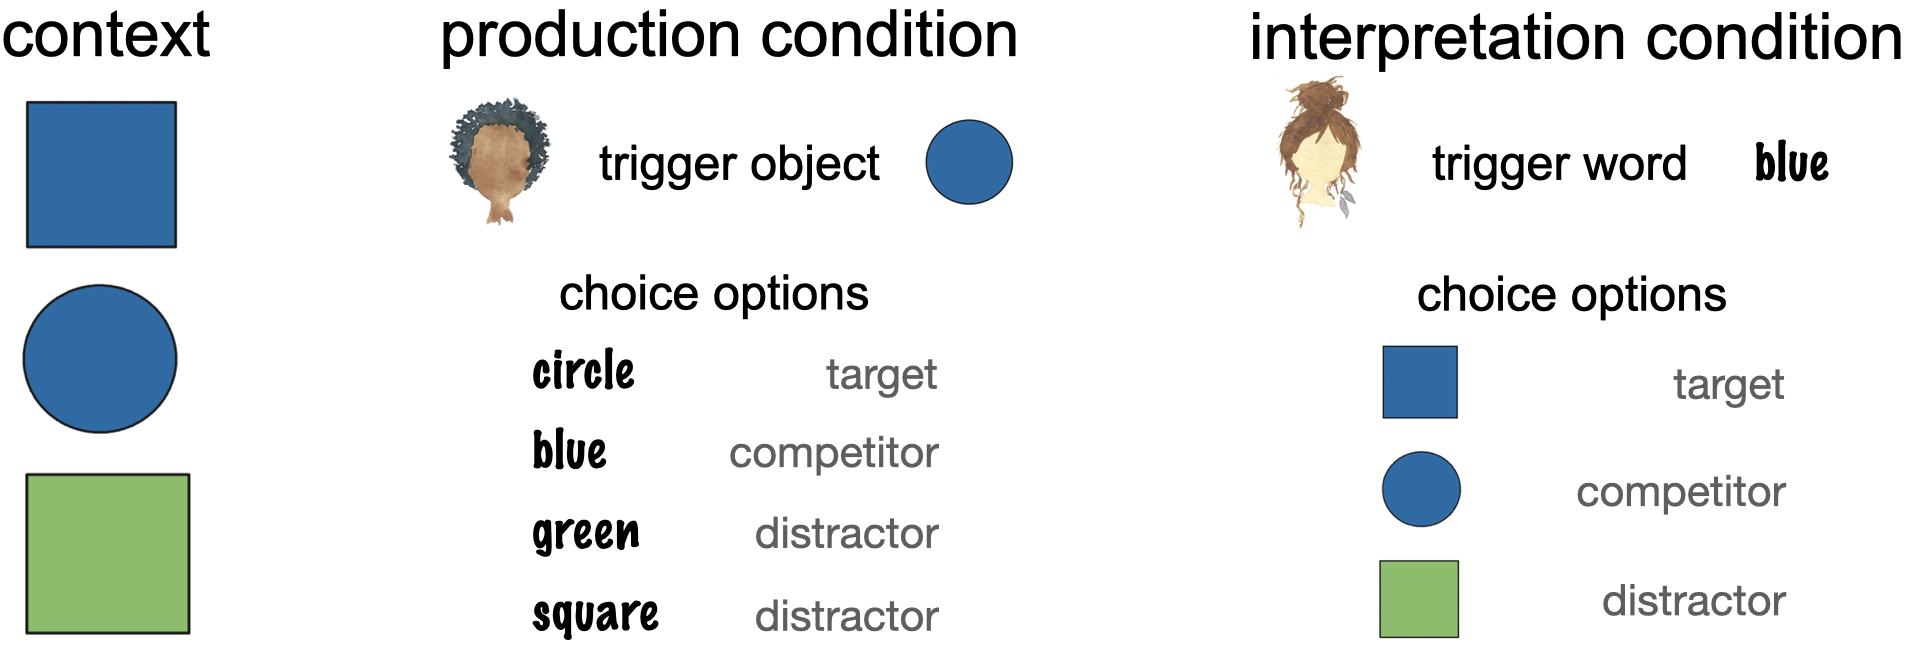
\includegraphics[width = 0.8\textwidth]{00-pics/reference-game.png}

  \caption{Structure of a reference game with human participants. Each trial consists of a set of objects, the so-called context. In production trials, participants choose a single word to describe a target object from the context. In interpretation trials, an object is selected as the likely object a trigger word referring to.}
  \label{fig:ref-game}
\end{figure}

To keep matters simple, we use an established, well-understood and austere experimental paradigm to test human decision making in abstract communicative tasks, so-called \textbf{reference games} \citep[e.g.,][]{FrankGoodman2012:Predicting-Prag,DegenFranke2013:Cost-Based-Prag,QingFranke2013:Variations-on-a,Frank2016:Rational-speech,SikosVenhuizen2021:Reevaluating-pr}.
A reference game consists of two players, a speaker and an interpreter, who jointly observe a set of objects, usually referred to as context (see Figure~\ref{fig:ref-game}).
In the \textbf{production condition}, the speaker is assigned a \emph{target object} from the context set which they have to describe to the interpreter.
In the \textbf{interpretation condition}, the interpreter observes a description, here called \emph{trigger word}, and chooses one of the objects from the context set.
The goal of the game is, for the speaker, to choose a description that enables the interpreter to choose the target object; and, for the interpreter, to guess correctly which object the speaker had in mind.

The example in Figure~\ref{fig:ref-game} is a standard case, which we will use throughout, where choices are informative about the pragmatic reasoning that decision makers engage in.
In this example, there are two features that differ across three objects (here shape and color).
One object shares both its color and shape with one other object, while the two other objects have one unique feature (e.g., being the only circle, or the only green object).
%
In a critical production trial, the target object to describe is one of the two objects with a unique feature.
The speaker has four words to choose from.
The \textbf{target utterance} is the word which uniquely describes the target object.
The \textbf{distractor utterance} is the word that is true of the target object, but also true of another object.
The other utterances, both of which are false of the target are \textbf{competitor utterance}.
%
In a critical interpretation trial, the trigger word is one that is true of two of the three objects.
If participants engage in pragmatic thought, they might reason that \emph{if} the speaker had wanted to refer to one of the two objects of which the trigger word is true (blue square and blue circle in Figure~\ref{fig:ref-game}), the speaker could have used a more informative word for exactly one of those two objects (``circle''), so they are more likely to refer to the \textbf{target object} (the blue square in Figure~\ref{fig:ref-game}).
The \textbf{competitor object} is the other object of which the trigger word is true.
The \textbf{distractor object} is the object of which the trigger word is false.

We replicated a simple reference game with human participants in which each trial instantiated the structure of the example shown in Figure~\ref{fig:ref-game}.
While previous reference games with human participants used pictorial representations of objects, and sometimes even pictorial representations of messages, we implemented a text-only version in order to be able to compare the predictions of LLMs for the exact same stimuli.
The experiment was realized as an online task using \texttt{magpie} \citep{FrankeJi:magpie:-Minimal}.\footnote{
  The code for the experiment can be found at \href{https://github.com/magpie-ea/magpie3-text-refgame}{https://github.com/magpie-ea/magpie3-text-refgame}, and a live version of the experiment can be tested at \href{https://magpie-ea.github.io/magpie3-text-refgame/}{https://magpie-ea.github.io/magpie3-text-refgame/}.
}


\subsection{Participants}
\label{participants}

A total of 302 participants were recruited via Prolific for monetary
compensation (\textsterling0.45, corresponding to roughly \textsterling 15.40 per hour).
All participants self-identified as native speakers of English.

\subsection{Materials \& design}
\label{materials-design}

We created 100 different items as stimulus material via a stochastic process.
Each item is a different textual description of a reference game with the same logical structure as the example from Figure~\ref{fig:ref-game}.
For each item, the context consisted of three objects.
Objects are defined by a triple of properties, namely a color, a shape and a texture.
For each property, there were four possible values, e.g., blue, green, red, and orange for color.
The sampled items differed in terms of the properties of the objects in the context set, and in terms of the order in which the objects and expression alternatives were presented in the text.
Figures~\ref{fig:refgame-screenshot-production} and \ref{fig:refgame-screenshot-interpretation} from Appendix~\ref{sec:scre-from-online} show example screenshots from the experiment.

\subsection{Procedure}
\label{procedure}

For each participant the experiment sampled four different items.
Participants first played two of these in the production condition, then the other two in the interpretation condition.


\subsection{Results}\label{results}

The overall distribution of choices that correspond to the target, competitor, and distractor states is shown in Figure~\ref{fig:refgame-counts} on the left.\footnote{
  The production condition actually has two distractor choices.
  Here and in the following, these are lumped together as a single category, also when modeling random errors in later models.
  This is a simplification but does not change anything of substance.}
It is interesting that the distractor options were chosen rather often.
We also see that the number of target choices is higher in the production condition than in the interpretation condition.
This is in line with previous experimental results on human reference games.
% \citep{QingFranke2013:Variations-on-a}.
For example, in previous forced-choice reference games with human participants with pictorial presentations of objects, \citet{QingFranke2013:Variations-on-a} observed the following proportions: $\tuple{0.882, 0.118, 0}$ in the production and $\tuple{0.492, 0.506, 0.003}$ in the interpretation condition (for 288 observations in each condition).

\begin{figure}
  \centering

    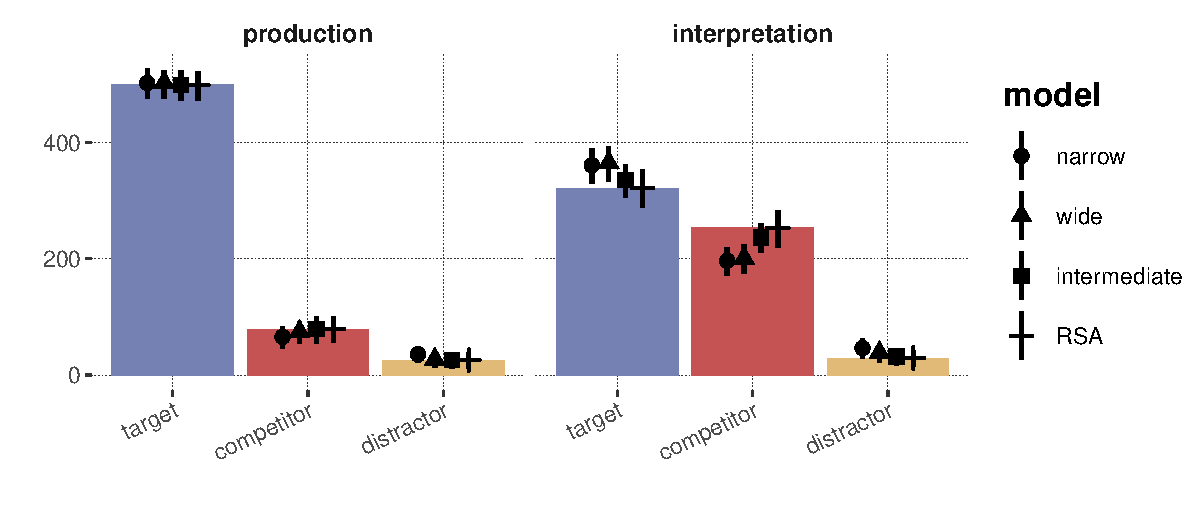
\includegraphics[width=0.9\linewidth]{00-pics/PPC-alpha-eps-model.pdf}

    \caption{Counts of choices from reference games with human participants (colored bars), with summary statistics from the posterior predictive distribution of three models (shapes and error bars).
      Shapes show the mean of the posterior predictive distributions of three models, differing in the scope of the item-level aggregation with respect to soft-maximizing and scaling.
      Error-bars show corresponding 95\% credible intervals of the posterior predictive.
    }
  \label{fig:refgame-counts}
\end{figure}


%%%%%%%%%%%%%%%%%%%%%%%%%%%%%%%%%%%%%%%%%%%%%%%%%%
\section{Model predictions from probabilistic pragmatics}
\label{sec:model-pred-from}
%%%%%%%%%%%%%%%%%%%%%%%%%%%%%%%%%%%%%%%%%%%%%%%%%%

Data from reference games with human participants have been variously analyzed with probabilistic models using inspiration from behavioral game theory \citep[e.g.,][]{DegenFranke2013:Cost-Based-Prag,QingFranke2013:Variations-on-a}, probabilistic Bayesian modeling \citep[e.g.,][]{FrankGoodman2012:Predicting-Prag,FrankeDegen2015:Reasoning-in-Re} or other forms of probabilistic modeling \citep[e.g.,][]{GattGompel2013:Are-we-Bayesian}.
Common to these approaches is that they derive or define, based on some explicit conceptual motivation, a parameterized stochastic policy, $P_{S}(u \mid s; \theta_{S})$, modulated by parameters $\theta_{S}$, for a speaker's choice of expression or utterance $u$ given a referent or state $s$, which the speaker wants to communicate;
and a stochastic listener policy, $P_{L}(s \mid u; \theta_{L})$, capturing the probability of choosing a referent $s$ for utterance $u$.

As a concrete example, we introduce the Rational Speech Act (RSA) model first described in this form by \citet{FrankGoodman2012:Predicting-Prag} \citep[for overview see][]{FrankeJager2015:Probabilistic-p,GoodmanFrank2016:Pragmatic-Langu,StevensBenz2018:Game-Theoretic-,ScontrasTessler2021:A-practical-int,Degen2023:The-Rational-Sp}.
The RSA model defines pragmatic reasoning as a sequence of iterated (soft-)optmization of policies, grounding out in literal interpretation.
If $\mathfrak{L}(s,u) \mapsto \set{0,1}$ is a semantic meaning function mapping each pair of state $s$ and utterance $u$ to a (binary) truth-value, and if $P_{s}$ is a prior over states, a literal listener policy is defined as:
%
\begin{align*}
 P_{L_{0}}(s \mid u) \propto \mathfrak{L}(s,u) P(s)\,.
\end{align*}
%
The pragmatic speaker soft-optimizes the choice of utterance to minimize the literal listener's surprisal for the to-be-communicated state:
%
\begin{align*}
  P_{S}(u_{i} \mid s, \alpha) & = \text{SoftMax}(\myvec{u}_{s}, \alpha)_{i}\,, \text{ where } \\
  \myvec{u}_{s} & = \tuple{\log P_{L_{0}}(s \mid u_{1}), \dots , \log P_{L_{0}}(s \mid u_{n})}\,.
\end{align*}
%
The softmax function \citep[c.f.,][]{FrankeDegen2023:The-softmax-fun} takes a vector of non-normalized scores $\myvec{s} = \tuple{s_{1}, \dots, s_{n}}$ and outputs a probability distribution $\myvec{p} = \tuple{p_{1}, \dots, p_{n}}$ in which odds are proportional to score differences, modulated by optimality parameter $\alpha$:
%
\begin{align*}
 \text{SoftMax}(\myvec{s}, \alpha) = \myvec{p}, \text{where } p_{i} \propto \expo \left (\alpha p_{i} \right )
\end{align*}
%
Finally, the pragmatic listener is defined as the policy resulting from applying Bayes rule, solving the inverse-problem for the previously defined speaker policy:
%
\begin{align*}
  P_{L}(s \mid u, \alpha) \propto  P_{S}(u \mid s, \alpha) \  P(s)
\end{align*}

\begin{figure}
  \centering
  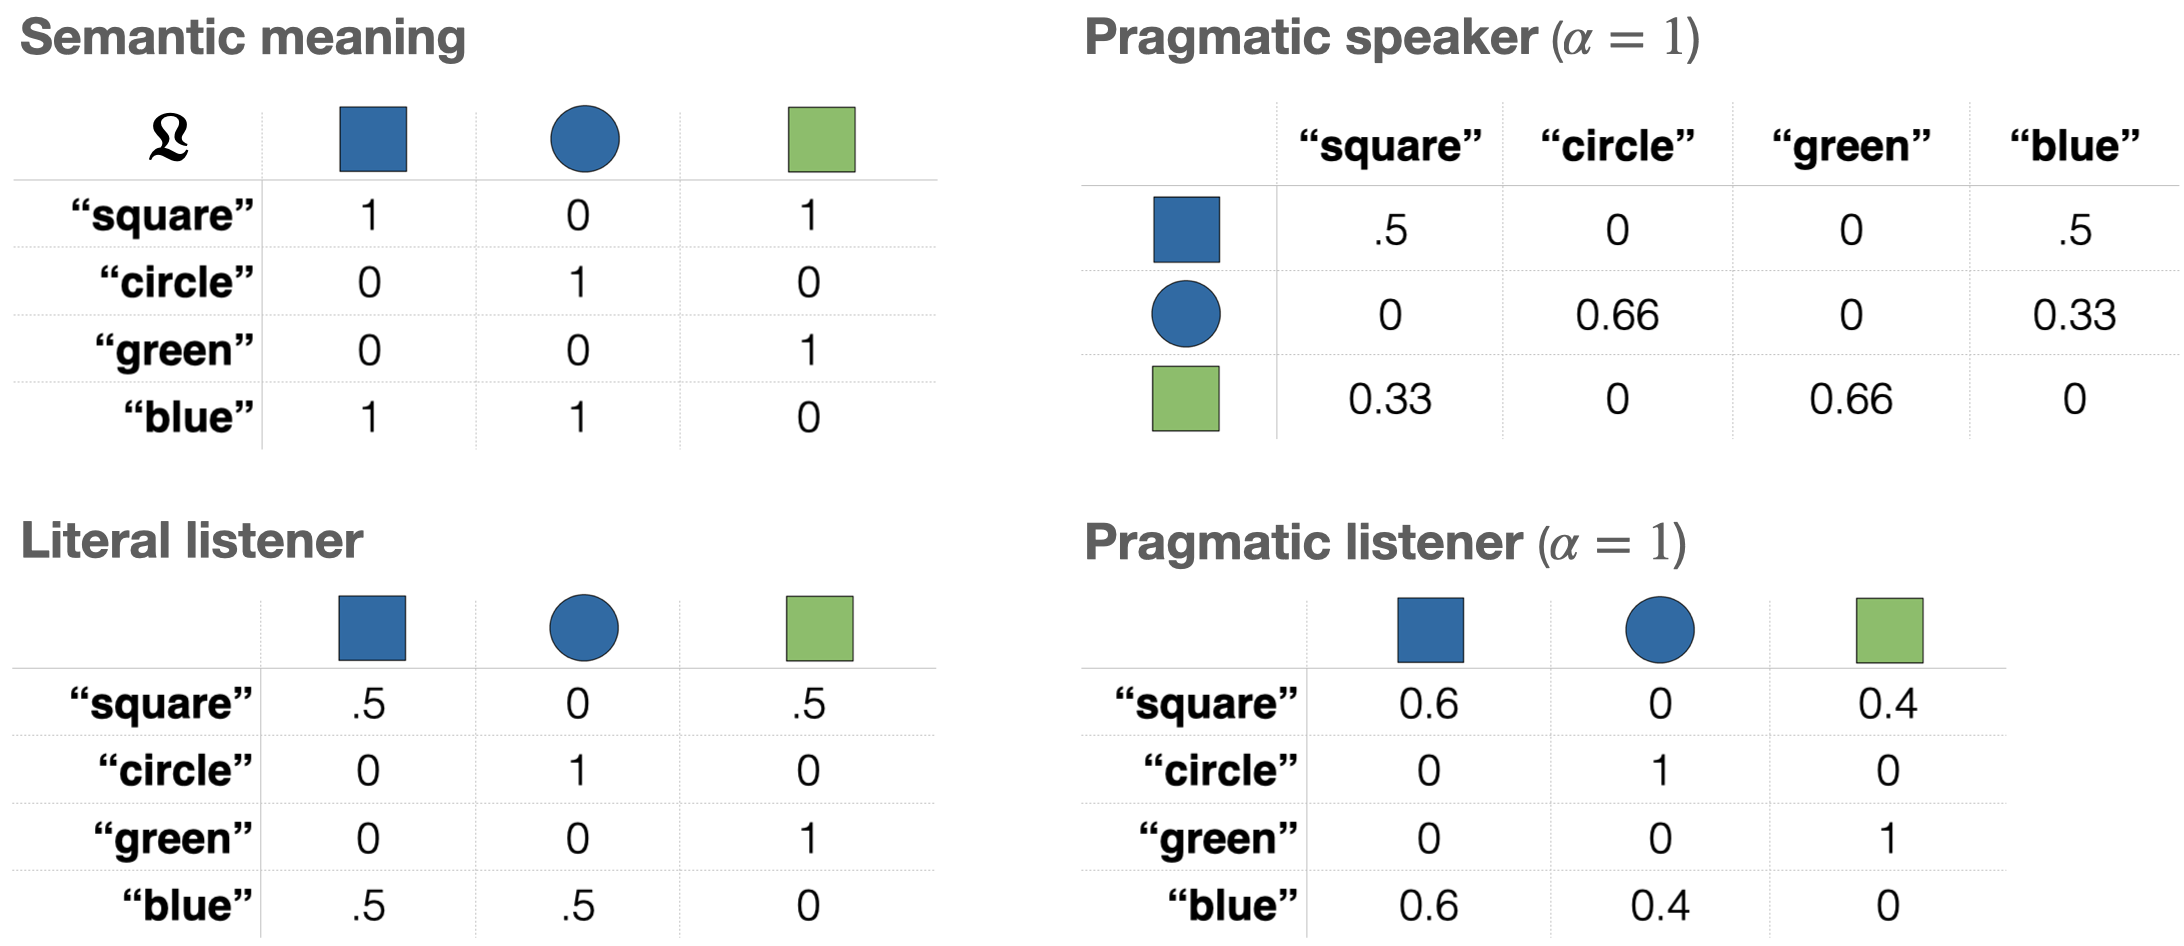
\includegraphics[width = 0.9 \textwidth]{00-pics/RSA-example.png}
  \caption{
    Example of predictions from the RSA model (with $\alpha=1$).
    The semantic meaning is shown as a matrix of binary truth-values.
    The policies of literal listener, pragmatic speaker and listener are calculated for uniform priors over state (referents), assume $\alpha=1$ and are shown as row-stochastic matrices.
  }
  \label{fig:RSA-example}
\end{figure}

Figure~\ref{fig:RSA-example} gives example calculations (assuming flat priors and $\alpha=1$) for the reference game from Figure~\ref{fig:ref-game}.
For $\alpha=1$, the model predicts that the probability of target, competitor and distractor options are $\tuple{\nicefrac{2}{3}, \nicefrac{1}{3}, 0}$ for the production, and $\tuple{0.6, 0.4, 0}$ for the interpretation condition.
Increasing $\alpha$ will increase the odds of target over competitor choices.
Yet, the model also predicts probability zero for distractor choices, so that the human data shown in Figur~\ref{fig:refgame-counts}e, where the distractor option was chosen in both conditions, would immediately rule out the model entirely.
It is therefore common to include a random error probability for each choice \citep[e.g.,][]{LeeWagenmakers2013:Bayesian-Cognit}, such as via Laplace smoothing: if $P_{r}(R_{l}, C, \alpha_{c})$ is the RSA model's probabilistic prediction for response category $R_{l}$ (target, competitor, or distractor) for condition $C$ (production or interpretation) and condition-specific optimality $\alpha_{c}$, the random-error smoothed prediction is:
\begin{align*}
  P_{r}(R_{l}, , C; \alpha_{c}, \epsilon_{c}) \propto P_{r}(R_{l}, C; \alpha_{c}) +  \frac{\epsilon_{c}}{3}\,,
\end{align*}
where $\epsilon_{c}$ is a (condition-specific) parameter giving the probability that a choice was made by randomly guessing.
The result is a four-parameter model, one pair of parameters per condition, which provides a likelihood function for the categorical choice data and so can be fitted to the data and compared against other probabilistic models providing a likelihood function for the same data.


%%%%%%%%%%%%%%%%%%%%%%%%%%%%%%%%%%%%%%%%%%%%%%%%%%
\section{LLM predictions for reference games}
\label{llm-predictions-for-reference-games}
%%%%%%%%%%%%%%%%%%%%%%%%%%%%%%%%%%%%%%%%%%%%%%%%%%

This section explores different ways of deriving a probabilistic likelihood function for the human data from a Large Language Model.
For a set-up in which the task descriptions and choice options are all text-based, predictions of LLMs at the item-level can be derived as a function of the (log) probabilities assigned to the continuations corresponding to each choice option after processing the task description.
The previous literature has shown that scoring longer sequences of text for an autoregressive LLM in terms of \emph{average next-token log probabilities}, or \emph{average log-probs} for short, gives improved predictions in relevant benchmark tests \citep[e.g.,][]{BrownMann2020:Language-Models}.
Using average log-probs for each answer option as a basic item-level score, there are at least three conceivable ways of deriving condition-level predictions by averaging over item-level variation (see Figure~\ref{fig:measures-overview}).
In the following, we first describe the different options of deriving LLM-based predictor terms.
We then compare all probabilistic models based on their adequacy of explaining the human choice data.

\begin{figure}
  \centering
  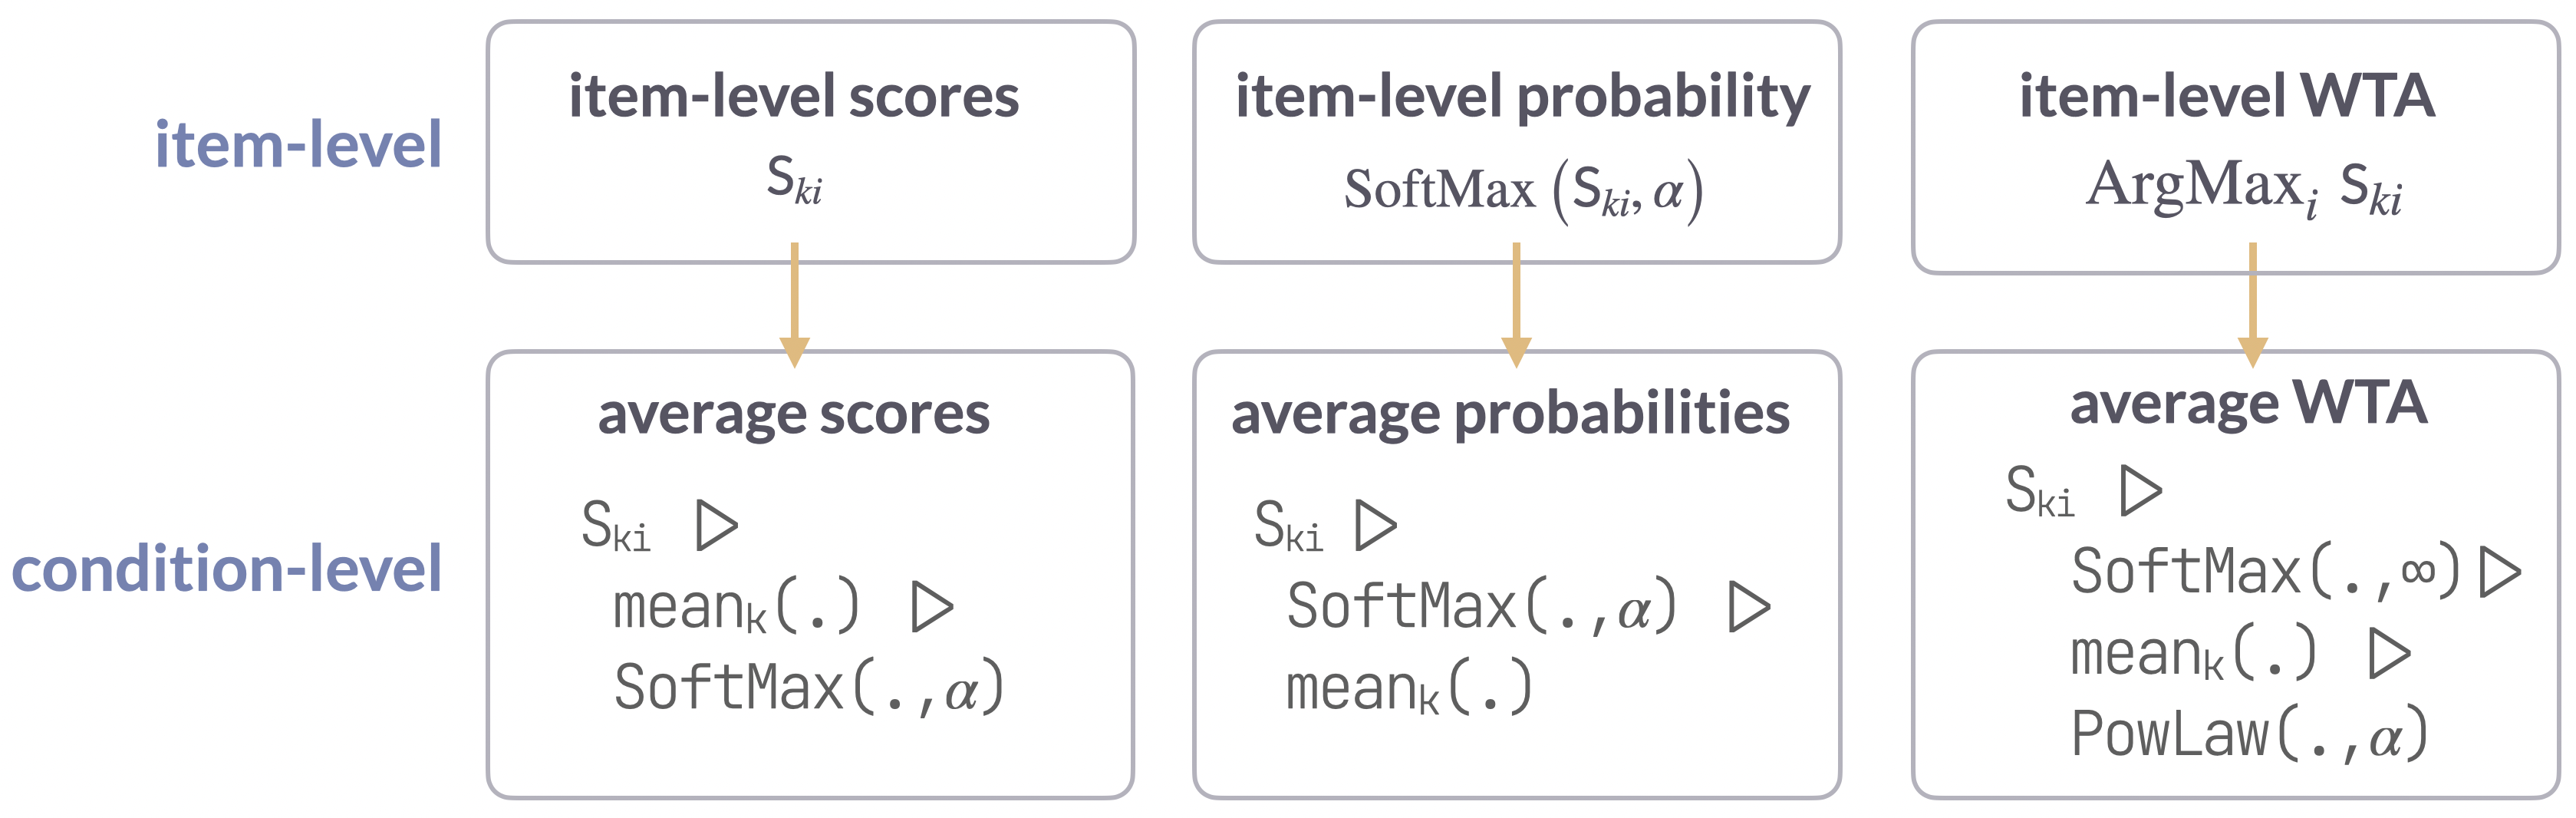
\includegraphics[width=0.9\textwidth]{00-pics/measures-overview.png}
  \caption{
    Schematic overview over three different approaches of obtaining condition-level predictions by aggregating over item-level scores.
    The basic item-level score is average next-word log probability.
    This can be taken as-is into averaging (narrow-scope aggregation), or first transformed from log- into probability-space, either with optimization before (wide scope) or after averaging (intermediate scope).
    The notation for the condition-level options uses pseudo-code to more clearly reflect the relevant operator scope differences (where triangles represent the pipe operator).
  }
  \label{fig:measures-overview}
\end{figure}

\subsection{LLM-based probabilistic predictions for forced-choice data}
\label{sec:notat--term}

Let $C$ be the experimental condition of interest (here: the production or interpretation condition).
Let \(\set{I_1, \dots I_m}\) be the multi-set of items that occurred in the human experiment for condition $C$.\footnote{
  By using a multi-set, which may contain a single task multiple times, we produce aggregate predictions for exactly the set of item that the participant group saw, which provides the most fitting counterpart to the human data.
}
Each item $I_{k}$ consists of a task description $T_{k}$ and $l$ choice options $O_{k1}, \dots, O_{kl}$, which are treated as textual continuations of the task description (see Appendix~\ref{sec:examples-items-llm} for an example).
For each item $I_{k}$, let $F(R_{l}, I_{k})$ be the choice option $O_{ki}$ that corresponds to \emph{response type} $R_{l}$ (here: target, competitor, distractor).\footnote{In the current set-up the response type ``distractor'' has two instantiations in the production condition. Since choice options are a single word in the production condition, for simplicity, we lump both of the distractor words together and treat them as a single option by taking the sum of the log-probabilities for both distractor words.}
We will define an item-level (non-normalized) score $S(O_{ki})$ for each choice option of a given item $k$, and use this to define a condition-level probabilistic predictions for response types by averaging over all items in a given condition.

\paragraph{Item-level score.}
If a choice option $O_{ki} = w$ is a single word, like in the production condition, an LLM's item-level prediction can simply be defined as the next-word log probability $\log P_{\text{LLM}} (w \mid T_{k})$.
If choice options are strings of more than one word, as in the interpretation condition, we follow the previous literature \citep[e.g.,][]{BrownMann2020:Language-Models} and define the \emph{item-level score} $S(O_{{ki}}, I_{k})$ for option $O_{ki} = w_{ki1}, \dots w_{kin}$ of item $k$, in terms of the average log-probs:
%
\begin{align*}
S(O_{ki}, I_{k}) =  \frac{1}{n} \sum_{j=1}^n \log P_{\text{LLM}} \left(w_{kij} \mid T_{k}, w_{ki1}, \dots, w_{ki(j-1)} \right)  \,.
\end{align*}
%
The item-level score of response type $R_{l}$ is $S(R_{l}, I_{k}) = S(F(R_{l}, I_{k}))$.

\paragraph{Condition-level predictions.}
Condition-level predictions are a probability distribution over response types, obtained from item-level scores $S(R_{l}, I_{k})$ by averaging over all items belonging to the relevant condition.
To map non-normalized scores $\myvec{s} = \tuple{s_{1}, \dots, s_{l}}$ to probabilities $\myvec{p} = \tuple{p_{1}, \dots, p_{l}}$ with different degrees of optimization, a common choice is the softmax function with optimality parameter $\alpha$, defined as:
%
\begin{align*}
 \text{SoftMax}(\myvec{s}, \alpha) = \myvec{p}, \text{where } p_{i} \propto \expo \left (\alpha p_{i} \right )
\end{align*}
%
The softmax function can furthermore be decomposed into a first step of mapping scores to probabilities, and subsequently reweighing probabilities via a power-law transformation:
%
\begin{align*}
  \text{SoftMax}(\myvec{s}, \alpha) & = \text{Pow}( \text{SoftMax}(\myvec{s}, 1) ; \alpha) \\
  \text{Pow}(\myvec{p} ; \alpha) & = \myvec{q}, \text{where } q_{i} \propto p_{i}^{\alpha}
\end{align*}
%
This means that there are three conceivable scope-sites for aggregating item-level information as shown in Figure~\ref{fig:measures-overview}.
Narrow-scope aggregation first aggregates the item-level scores, and then transposes the averages into (scaled) probabilities:
%
\begin{align*}
  % & \textbf{narrow-scope aggregation} \\
  & P_{n}(R_{l}, C ; \alpha) \propto \expo \left [  \alpha \ \frac{1}{m} \ \sum_{i = k}^{m} S(R_{l}, I_{k})  \right ]
    \tag*{\textcolor{gray}{[narrow-scope aggregation]}}
\end{align*}
%
Wide-scope aggregation, first transposes scores into probabilities, scales them and only aggregates over items last.
\begin{align*}
  % & \textbf{wide-scope aggregation} \\
  & P_{w}(R_{l}, C ; \alpha) \propto \frac{1}{m} \ \sum_{i = k}^{m} \frac{\expo \left( \alpha \ S(R_{l}, I_{k}) \right )}{ \sum_{l'} \expo \left( \alpha \ S(R_{l'}, I_{k}) \right )}
    \tag*{\textcolor{gray}{[wide-scope aggregation]}}
\end{align*}
%
Intermediate-scope aggregation performs item-level averaging after mapping scores onto probabilities (using softmax with $\alpha=1$), but before scaling (with a power-law transformation with variable $\alpha$):
\begin{align*}
  % & \textbf{intermediate-scope aggregation} \\
  & P_{i}(R_{l}, C ; \alpha) \propto  \left [ \frac{1}{m} \ \sum_{i = k}^{m} \frac{\expo \left( S(R_{l}, I_{k}) \right )}{ \sum_{l'} \expo \left( S(R_{l'}, I_{k}) \right )} \right ]^{\alpha}
    \tag*{\textcolor{gray}{[intermediate-scope aggregation]}}
\end{align*}

All three condition-level predictors coincide when there is only one item, of course.
For more items, wide-scope and intermediate-scope aggregation coincide when $\alpha = 1$.
In all other cases, the predictors are not guaranteed to be identical.
Conceptually, the main difference is what each measure considers to be the basic item-level unit to aggregate over.
Narrow-scope aggregation considers raw scores, not \emph{not} probabilistic predictions at the item level.
Wide-scope aggregation considers $\alpha$-optimized probabilities at the item level, which is compatible with a procedure of sampling, via softmax decoding, item-level answer options.
Similarly, intermediate-scope aggregation is also compatible with a sampling based picture, but would use pure decoding (without $\alpha$-optimization) at the item level.

\subsection{Model fitting, criticims \& comparison}
\label{sec:model-fitting}

Parameterized predictions $P_{m}(R_{l}, C ; \alpha_{c})$ for models $m \in \set{n,w,i,r}$, where $r$ is the RSA model introduced in Section~\ref{sec:model-pred-from}, can be assessed in the light of the empirical data from human participants with the usual tools of Bayesian data analysis \citep[e.g.][]{GelmanCarlin2014:Bayesian-Data-A,McElreath2016:Statistical-Ret,Lambert2018:A-Students-Guid}.
For each condition $C$ (production and interpretation), each model has a free optimality parameter $\alpha_{c}\sim \text{log-Normal}(0.5,1)$ with a log-Normal prior.
Following the rationale from Section~\ref{llm-predictions-for-reference-games}, we also assume that each model has one epsilon parameter per condition, $\epsilon_{c}$, which accounts for random errors in the human data via Laplace smoothing, with a prior $\epsilon_{c} \sim \text{Beta}(1,5)$ favoring small values.
The resulting likelihood function for model $m$ and data from condition $C$ is a multinomial distribution with predictor for response $R_{l}$ given by:
%
\begin{align*}
  P_{m}(R_{l}, C; \alpha_{c}, \epsilon_{c}) \propto P_{m}(R_{l}, C; \alpha_{c}) +  \frac{\epsilon_{c}}{3}
\end{align*}

Using Stan \citep{Team2023:The-Stan-Core-L} for Bayesian inference, we obtain estimates of posterior credible values of each $\alpha_{c}$ and $\epsilon_{c}$ for each model.
The usual Bayesian summary statistics for posteriors over model parameters are shown in Figure~\ref{fig:posterior-stats}.

\begin{table}[ht]
  \centering

  % 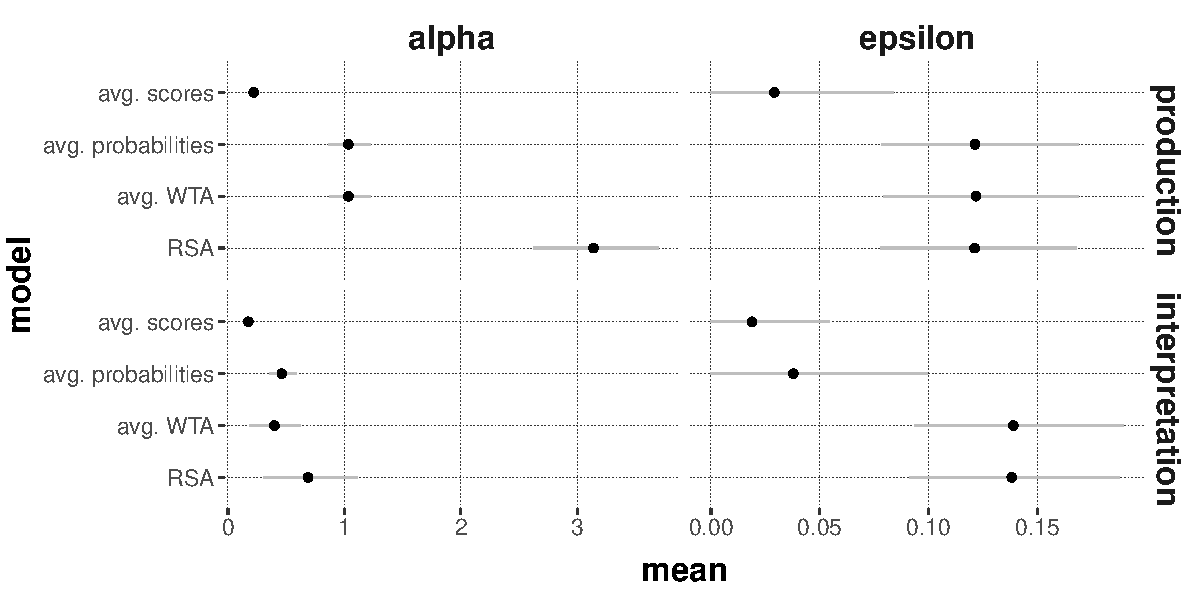
\includegraphics[width=0.9\linewidth]{00-pics/posterior-stats.pdf}

  \begin{tabular}{llllcr}
    \toprule \addlinespace[1ex]
    model        & condition      & Parameter  & $|$95\% & mean & 95\%$|$ \\
    \midrule  \addlinespace[1ex]
    narrow       & production     & $\alpha$   & 0.19    & 0.22 & 0.26 \\
                 &                & $\epsilon$ & 0.00    & 0.04 & 0.11 \\
                 & interpretation & $\alpha$   & 0.15    & 0.18 & 0.20 \\
                 &                & $\epsilon$ & 0.00    & 0.02 & 0.06 \\ \addlinespace[0.75ex]
    intermediate & production     & $\alpha$   & 0.86    & 1.04 & 1.22 \\
                 &                & $\epsilon$ & 0.08    & 0.13 & 0.18 \\
                 & interpretation & $\alpha$   & 0.36    & 0.48 & 0.60 \\
                 &                & $\epsilon$ & 0.00    & 0.05 & 0.12 \\ \addlinespace[0.75ex]
    wide         & production     & $\alpha$   & 0.22    & 2.69 & 8.79 \\
                 &                & $\epsilon$ & 0.08    & 0.13 & 0.19 \\
                 & interpretation & $\alpha$   & 0.19    & 1.08 & 6.03 \\
                 &                & $\epsilon$ & 0.00    & 0.06 & 0.18 \\ \addlinespace[0.75ex]
    RSA          & production     & $\alpha$   & 2.59    & 3.16 & 3.71 \\
                 &                & $\epsilon$ & 0.08    & 0.13 & 0.18 \\
                 & interpretation & $\alpha$   & 0.24    & 0.66 & 1.07 \\
                 &                & $\epsilon$ & 0.10    & 0.15 & 0.20 \\ \addlinespace[0.25ex]
    \bottomrule \\
  \end{tabular}

  \caption{
    Summary statistics of posterior samples.
    Number indicate estimates for lower and upper bounds of 95\% credible intervals and the posterior means.
    \mf{maybe not necessary, but can we explain the high values for $\alpha$ in the wide model?}
  }
  \label{fig:posterior-stats}
\end{table}

To assess goodness-of-fit, Figure~\ref{fig:refgame-counts} shows summary statistics (means and 95\% credible intervals) for each model's posterior predictive distribution, i.e., the model's predictions about data of the same size and structure as the training data.
As a minimal bar, we would require a model trained on observed data $D_{\text{obs}}$ to not be surprised by $D_{\text{obs}}$.
Figure~\ref{fig:refgame-counts} shows that only the theoretical model (RSA) and the intermediate-scope model passes this ``visual posterior predictive check'' for both conditions; the other two models both overpredict the target choice rate and underpredict the competitor choice rate.
To corroborate the visual impression, Table~\ref{tab:Bppp-values} shows sample-based estimates of Bayesian posterior predictive $p$-values, using likelihood of the observed data as a test statistics.
These values approximate the probability that a model trained on $D_{\text{obs}}$ would predict future data of the same size and format that is at least as unlikely as the data $D_{\text{obs}}$ itself.
Low values therefore indicate that the trained model would be highly surprised by the data it was trained on; an indication that it failed to capture something essential about the training data.
Consequently, the results from Table~\ref{tab:Bppp-values} suggest that the narrow-scope model fails on the interpretation data, and is at most borderline compatible with the production data; that the wide-scope model is able to reproduce the production data, but fails on the interpretation data; and that only the intermediate-scope model is able to fully recover the data from both conditions.

\begin{table}[ht]
\centering

% \begin{tabular}{lrr}
%   \toprule
%   model        & production & interpretation \\ \midrule
%   narrow       & 0.05       & 0.00 \\
%   wide         & 0.51       & 0.00 \\
%   intermediate & 0.49       & 0.26 \\
%   RSA          & 0.49       & 0.52 \\
%   \bottomrule \\
% \end{tabular}

\begin{tabular}{lrrrr}
  \toprule
  & narrow & wide & intermediate & RSA \\ \midrule
  production & 0.05 & 0.51 & 0.49 & 0.49 \\
  interpretation & 0.00 & 0.00 & 0.26 & 0.52 \\ \bottomrule \\
\end{tabular}


\caption{Sample-based estimates of Bayesian posterior predictive $p$-values for each model and each condition, based on likelihood of the observed data as test statistic.}
\label{tab:Bppp-values}
\end{table}

These results tell us that not all ways of deriving condition-level predictions by averaging over item-level variation are equally good.
Some approaches clearly fail basic checks for statistical goodness-of-fit.
On the positive side, we also find that there is at least one model with predictors based on LLM-measures, namely the intermediate-scope model, which is able to recover the patterns in the data.
In other words, there is a way of deriving predictor values for condition-level forced-choice probabilities from an LLM such that, when fed into a common linking function (here with parameters $\alpha$ for optimization and $\epsilon$ for random error), the human choice probability can be reconstructed faithfully in its entirety.\footnote{
  A potential worry is that the intermediate-scope model is trivial in the sense that it could have predicted \emph{any} data observation.
  Appendix~\ref{sec:range-prior-pred} shows that this is not the case.
}
This implies that using LLM predictors for probabilistic predictions, such as in a neuro-symbolic model, might be possible if embedded in the proper link functions and if item-level variation is averaged out in the right way.


%%%%%%%%%%%%%%%%%%%%%%%%%%%%%%%%%%%%%%%%%%%%%%%%%%
\section{Item-level predictions}
\label{sec:item-level-pred}
%%%%%%%%%%%%%%%%%%%%%%%%%%%%%%%%%%%%%%%%%%%%%%%%%%

The ability to predict a condition-level averages is useful for applications, and may also be theoretically insightful.
Nevertheless, for human data, averages over item- or individual-level variation can also be misleading \citep[e.g.,][]{StanovichWest2000:Individual-diff,EstesMaddox2005:Risks-of-Drawin,HaafRouder2019:Some-do-and-som}, as aggregate patterns may be artifacts of systematic variation at the subject- or item-level.
LLMs do not make individual-level predictions, at least not without further intervention, such as special prompting.
But the question remains whether the variation in item-level predictions made by LLMs is reflected in the human data.

To address this question, we fit a model to the human data at the item-level.
The data to be explained is the set of all response type counts $\tuple{t_{k}, c_{k}, d_{k}}$ for each item $I_{k}$.
The model's predictions for the data from item $I_{k}$ from condition $C$ (production or interpretation) are:
%
\begin{align*}
  P_{\text{item}}(R_{l}, C, I_{k}, \alpha_{c}, \epsilon_{c}) \propto \frac{\expo \left( \alpha_{c} \ S(R_{l}, I_{k}) \right )}{ \sum_{l'} \expo \left( \alpha_{c} \ S(R_{l'}, I_{k}) \right )} + \epsilon_{c}
\end{align*}
%
In words, we use a single pair or parameters $\alpha_{c}$ and $\epsilon_{c}$, one for each condition, take the LLM's item-level scores for each item, and derive the response probabilities in the exact same way as before.

Figure~\ref{fig:item-level-obs-pred} shows that the item-level LLM predictor predicts variance which is not borne out by the human data.
Concretely, the plot shows, for each item, mean posterior estimates of the model's predicted probability of choosing the target option ($x$-axis), together with the observed proportion of target choices in the human data.
There is ample variation in the model predictions, especially visible in the production condition, owing to the fact that the item-level scores of the LLM sometimes clearly favor another option than the target choice.
So, the model itself predicts systematic variability at the item level.
The human data, too, show variability at the item-level, but there is no (visual) indication that the item-level variability predicted by the LLMs is borne out by the human data.
In fact, sampling-based approximations of Bayesian posterior predictive $p$-values for the by-item analysis are very low (0.0001 for production, 0 for interpretation), suggesting that the unaggregated item-level LLM predictions are inadequate predictors of the human data.
In contrast, using the global, item-independent RSA model predictions to fit the item-level data, we obtain estimates of posterior predictive $p$-values that do not discredit the model ($~0.338$ for each condition).
These results suggest that LLM-based probabilistic predictions may imply item-level variance that is not attested in the human data.

\begin{figure}
  \centering

  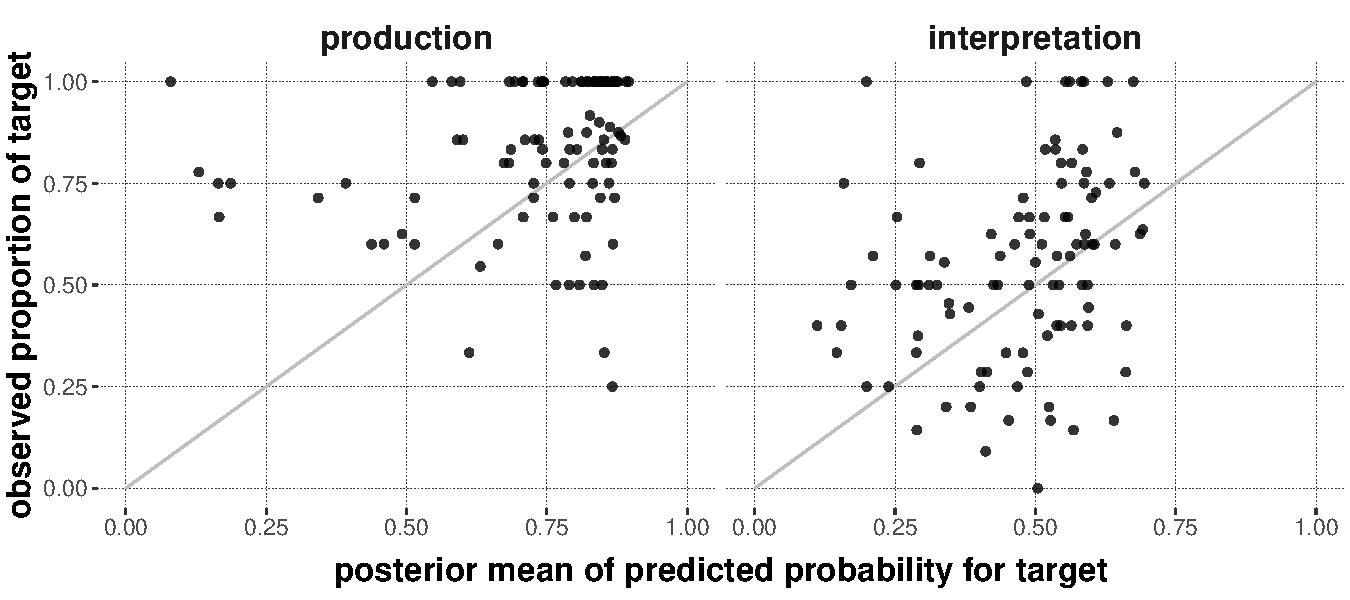
\includegraphics[width = 0.9\linewidth]{00-pics/item-combined-obs-pred.pdf}

  \caption{
    Item-level prediction-observation plot.
    Each dot represents an item.
    The $x$-coordinate represents the mean of the posterior prediction for the target choice probability for the given item.
    The $y$-coordinate represents the observed proportion of target choices for that item.
    The gray line (identity function) is the ideal prediction.
  }
  \label{fig:item-level-obs-pred}
\end{figure}


%%%%%%%%%%%%%%%%%%%%%%%%%%%%%%%%%%%%%%%%%%%%%%%%%%
\section{Conclusion}
\label{conclusion}
%%%%%%%%%%%%%%%%%%%%%%%%%%%%%%%%%%%%%%%%%%%%%%%%%%

It is not entirely ludicrous to use numerical predictions from LLMs are
part of predictive probabilistic models. But we have to be careful.
Ideally, we average out over low-level variation, such as from order of
presentation or similar ``nuisance,'' at least as long as we do not
understand what causes this variation in the predictions of models and
further research that investigates when exactly this variation accords
with empirically observed patterns.

This also implies that we should likely \emph{not} (yet) aspire to use
LLMs are models or individual- or item-level predictors.

( {TODO: rethink conclusion})

{to be continued}

\newpage
\appendix


%%%%%%%%%%%%%%%%%%%%%%%%%%%%%%%%%%%%%%%%%%%%%%%%%%
\section{Screenshots from the online experiment with human participants}
\label{sec:scre-from-online}
%%%%%%%%%%%%%%%%%%%%%%%%%%%%%%%%%%%%%%%%%%%%%%%%%%

Figure~\ref{fig:refgame-screenshot-production} shows a trial from the production condition, Figure~\ref{fig:refgame-screenshot-interpretation} one for the interpretation condition of the online experiment.

\begin{figure}[H]
  \centering
  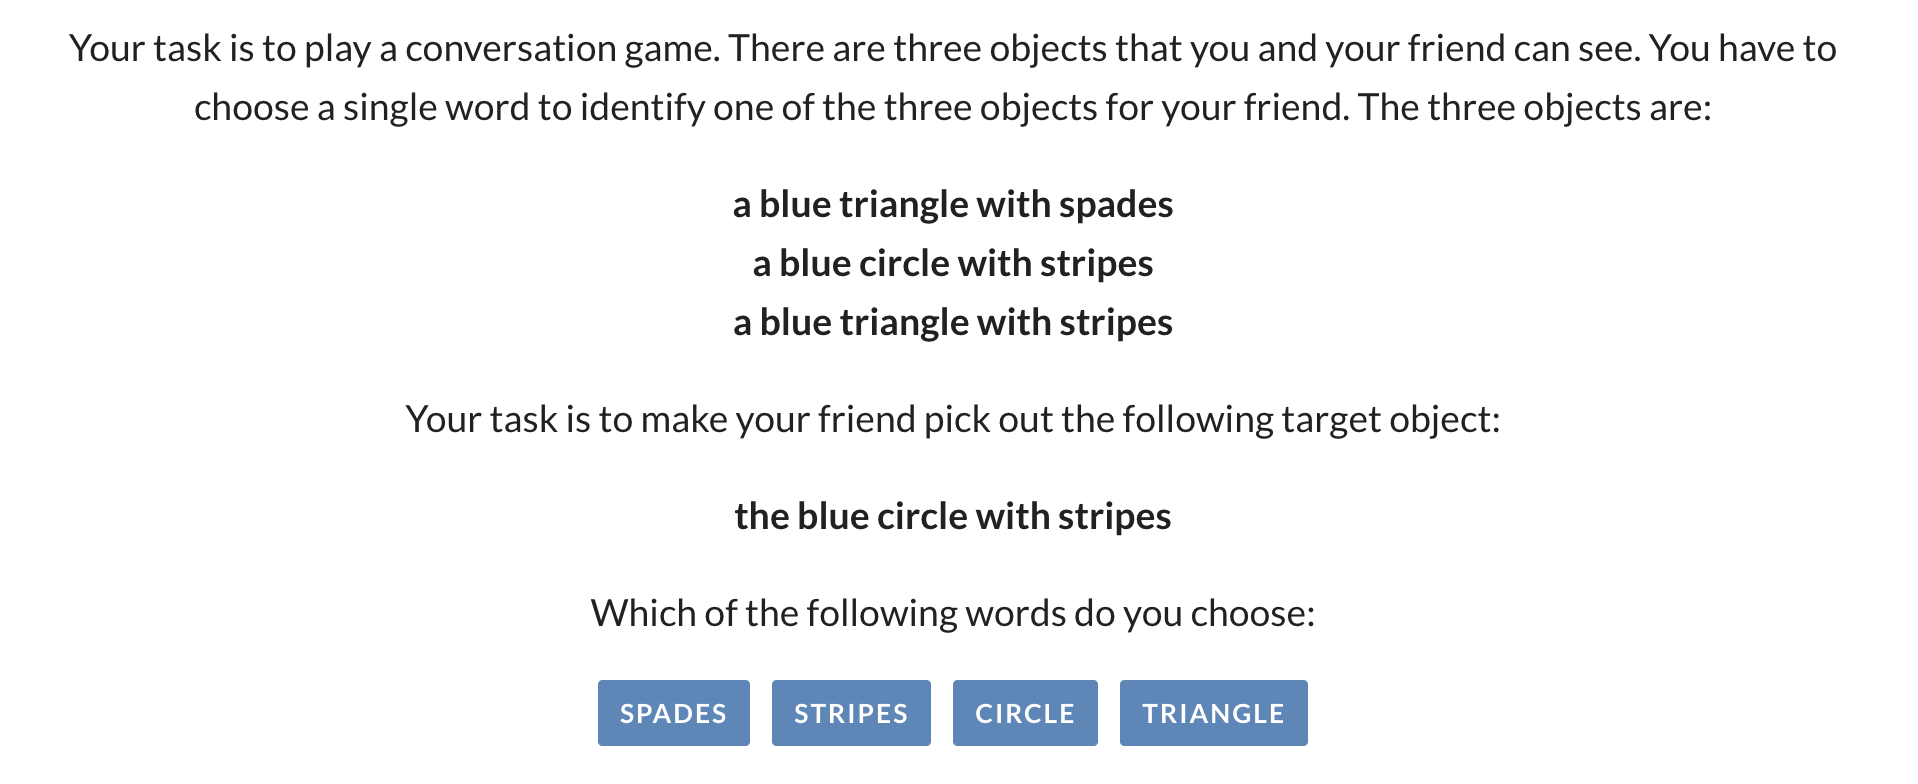
\includegraphics[width = 0.8\textwidth]{00-pics/refgame-production.png}

  \caption{Screen shot from a production trial of the online experiment.}
  \label{fig:refgame-screenshot-production}
\end{figure}

\begin{figure}[H]
  \centering
  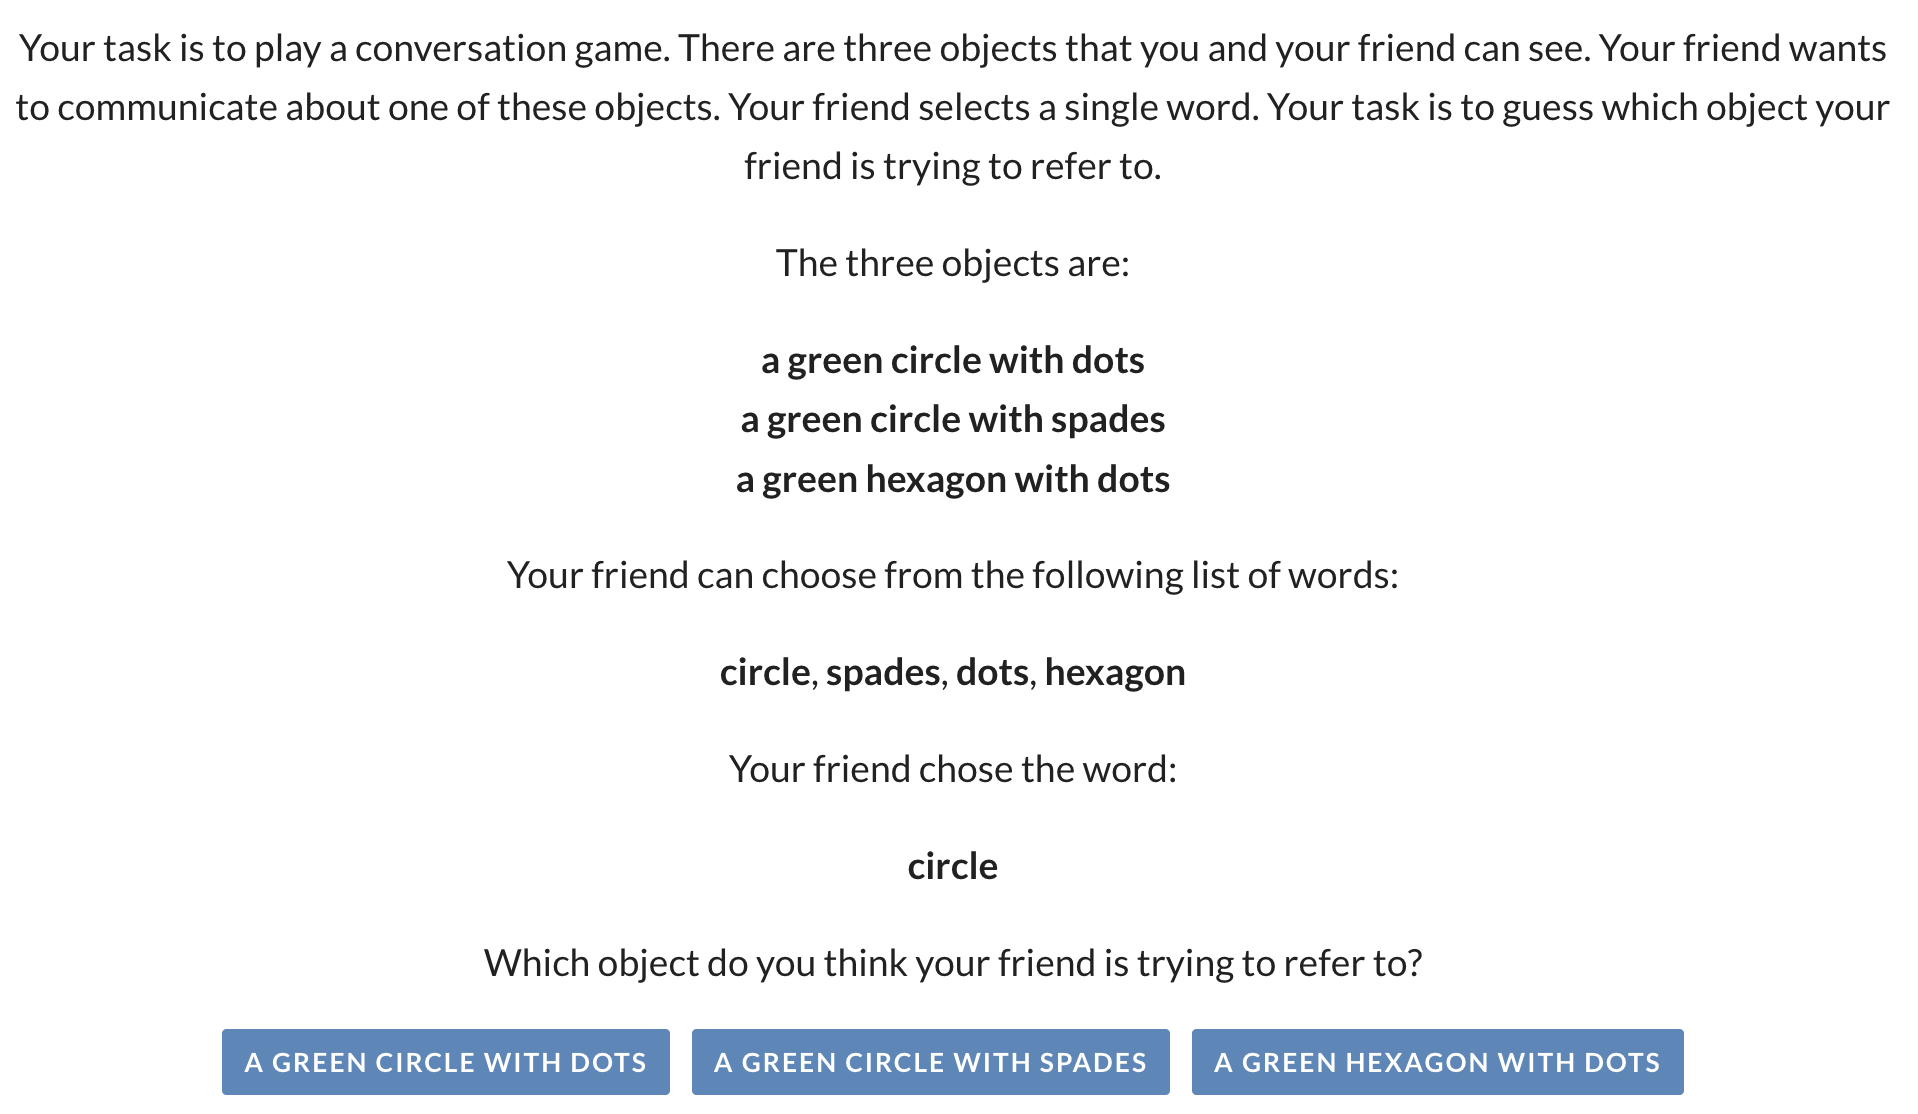
\includegraphics[width = 0.8\textwidth]{00-pics/refgame-interpretation.png}

  \caption{Screen shot from an interpretation trial of the online experiment.}
  \label{fig:refgame-screenshot-interpretation}
\end{figure}

\section{Example item for the LLM experiment}
\label{sec:examples-items-llm}

The text-based input for the LLM predictions mirrors the text in the human experiment, except that the LLM input also lists the set of all available choice options (which for the human experiment is unnecessary since this information is given by the buttons for the forced-choice selection).
For example, the task description $T_{k}$ for the item that corresponds to the production trial shown in Figure~\ref{fig:refgame-screenshot-production} is shown below (the actual input has no line breaks in the first paragraph):

\begin{verbatim}
Your task is to play a conversation game. There are three objects that
you and your friend can see. You have to choose a single word to identify
one of the three objects for your friend.

The three objects are:

a blue triangle with spades
a blue circle with stripes
a blue triangle with stripes

Your task is to make your friend pick out the following target object:

the blue circle with stripes

Which of the following words would you choose:

spades
stripes
circle
triangle

Your answer:

I would choose the word
\end{verbatim}


%%%%%%%%%%%%%%%%%%%%%%%%%%%%%%%%%%%%%%%%%%%%%%%%%%
\section{Range of prior predictions of intermediate-scope model}
\label{sec:range-prior-pred}
%%%%%%%%%%%%%%%%%%%%%%%%%%%%%%%%%%%%%%%%%%%%%%%%%%

It may seem that, given the freedom to adjust optimization $\alpha$ and random guessing rate $\epsilon$, some models might be able to explain \emph{any} data observation.
The intermediate-scope model, which was not discredited by model criticism in terms of recovery-based posterior predictive checks, is not trivial in this sense.
Figure~\ref{fig:prediction-range} shows the range of predictions that the intermediate-scope model is, in principle, capable of making (for the whole possible range of \(\alpha\) and \(\epsilon\) values, disregarding Bayesian priors).
There are distributions over response types which the model does not explain predict \emph{ex ante}.
For example, the model does not predict cases where the number of competitor choices is almost as high as the number of target choice, as would be the case if participants would consistently \emph{not} engage in pragmatic reasoning.


\begin{figure}[t]
  \centering

  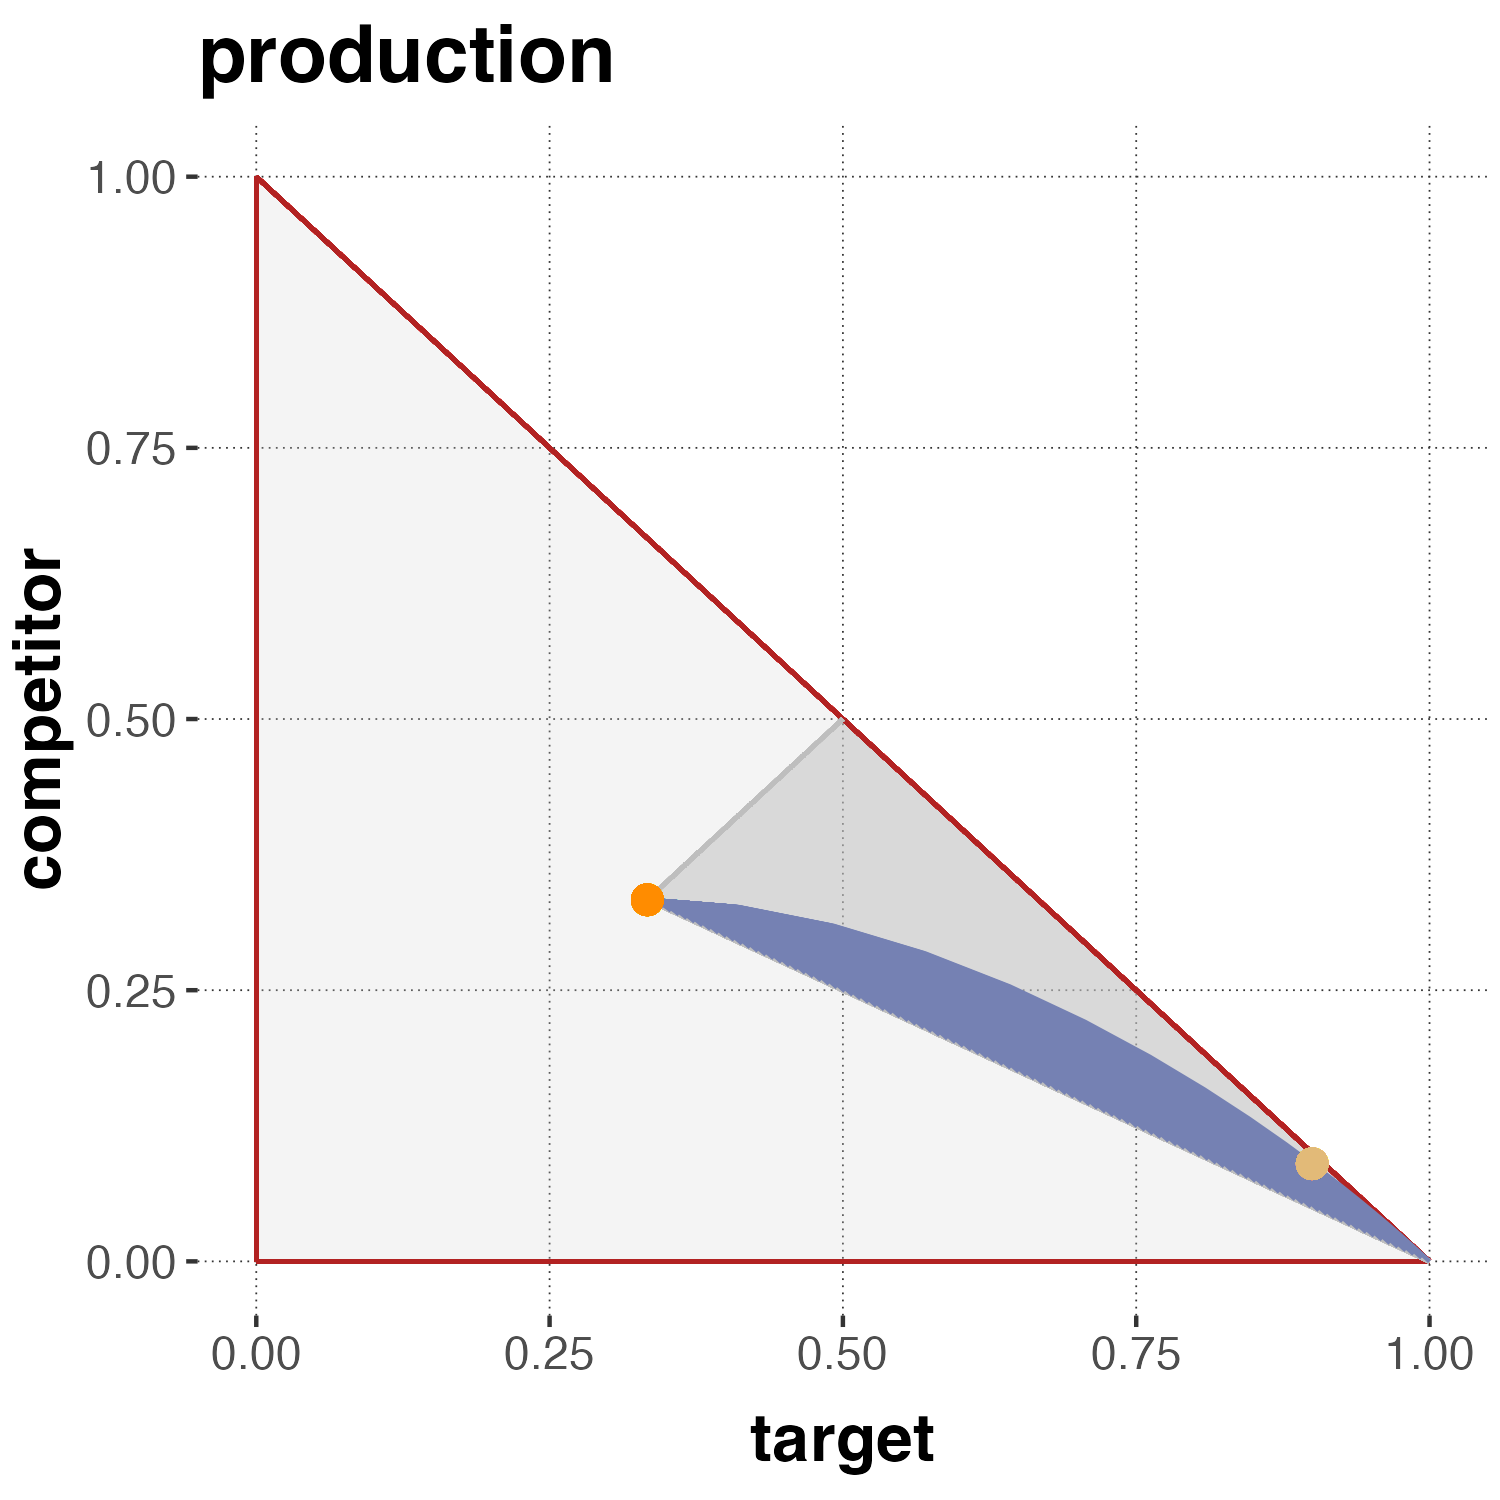
\includegraphics[width=0.45\textwidth]{00-pics/prediction-range-prod.png}
  %
  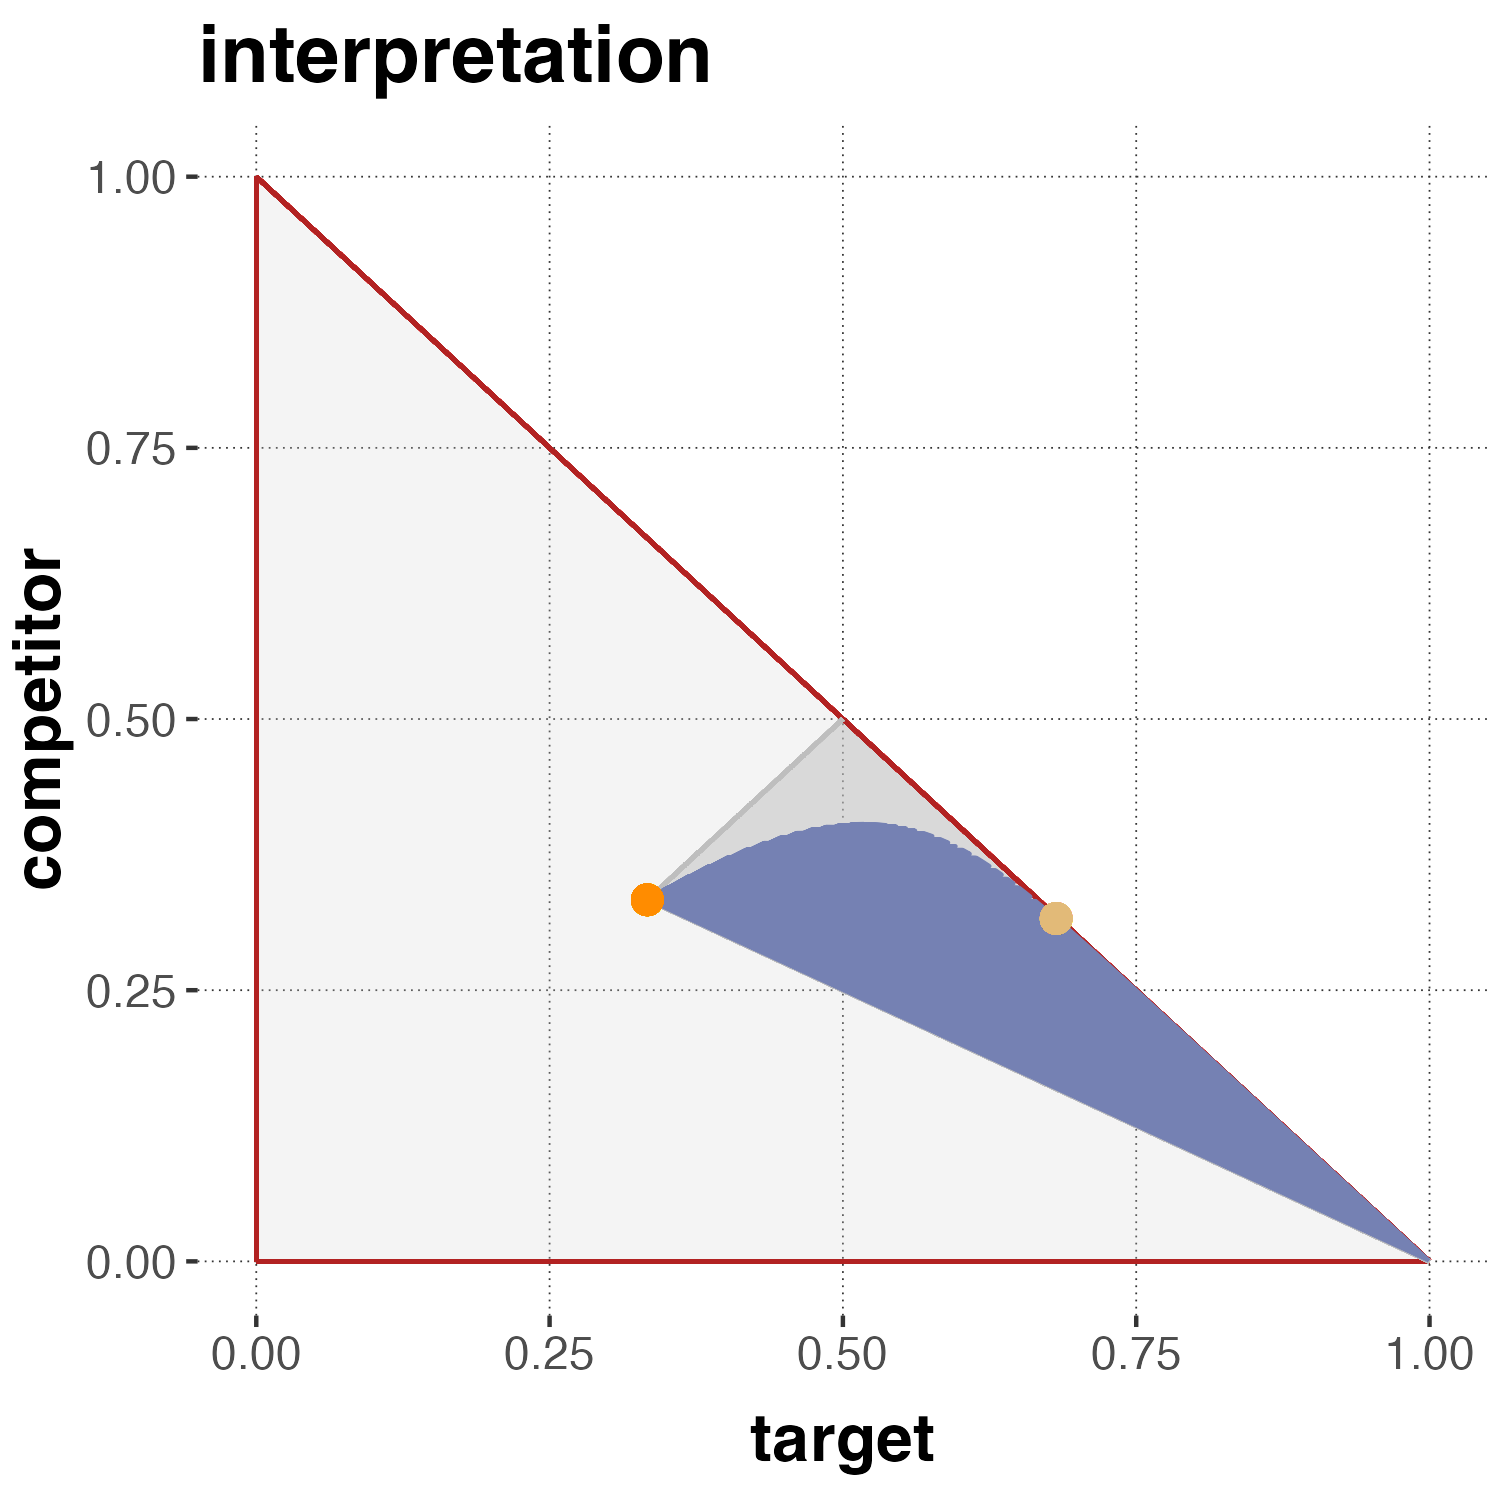
\includegraphics[width=0.45\textwidth]{00-pics/prediction-range-inter.png}

  \caption{
    Range of predictions the intermediate-scope model makes for any pair of parameter values $\alpha_{c}$ and $\epsilon_{c}$.
    The light gray triangle with the red boundary is the probability simplex, i.e., the space of all possible 3-place probability vectors.
    The darker gray area in gray boundary lines is the subspace that is compatible with the ordering that the probability of choosing the target is bigger than that of the competitor, which in turn is bigger than that of the distractor.
    The blue area is the subspace of probabilistic predictions the intermediate-scope model makes under any value of its parameters.
    The orange dot in the middle is the ``Laplace point'' of equal probability for all three options, which the model predicts for $\alpha=0$ or $\epsilon=1$.
    The yellow dot is the ``vanilla prediction'' for $\alpha_{c}=1$ and $\epsilon_{c}=0$.
  }
  \label{fig:prediction-range}
\end{figure}


\printbibliography[heading=bibintoc]


\end{document}
